\documentclass[10pt, compress, aspectratio=169]{beamer}

\usetheme[numbering=fraction, progressbar=none, titleformat=smallcaps]{metropolis}
\usepackage{booktabs}
\usepackage{array}
\usepackage{listings}
\usepackage{graphicx}
\usepackage[scale=2]{ccicons}
\usepackage{url}
\usepackage{relsize}
\usepackage{wasysym}

\usepackage{pgfplots}
\usepgfplotslibrary{dateplot}

\lstset{ %
  backgroundcolor={},
  basicstyle=\ttfamily\footnotesize,
  breakatwhitespace=true,
  breaklines=true,
  captionpos=n,
  commentstyle=\color{orange},
  escapeinside={\%*}{*)},
  extendedchars=true,
  frame=n,
  keywordstyle=\color{orange},
  language=C++,
  rulecolor=\color{black},
  showspaces=false,
  showstringspaces=false,
  showtabs=false,
  stepnumber=2,
  stringstyle=\color{gray},
  tabsize=2,
  keywords={thrust,plus,device_vector, copy,transform,begin,end, copyin,
  copyout, acc, \_\_global\_\_, void, int, float, main, threadIdx, blockIdx,
  blockDim, if, else, malloc, NULL, cudaMalloc, cudaMemcpy, cudaSuccess,
  cudaGetLastError, cudaDeviceSynchronize, cudaFree, cudaMemcpyDeviceToHost,
  cudaMemcpyHostToDevice, const, data, independent, kernels, loop,
  fprintf, stderr, cudaGetErrorString, EXIT_FAILURE, for, dim3},
  otherkeywords={::, \#pragma, \#include, <<<,>>>, \&, \*, +, -, /, [, ], >, <}
}

\renewcommand*{\UrlFont}{\ttfamily\smaller\relax}

\graphicspath{{images/}}

\title{SSH and OpenSSH}
\author{\footnotesize Rodrigo Siqueira \\ {\scriptsize siqueira@ime.usp.br}}
\institute{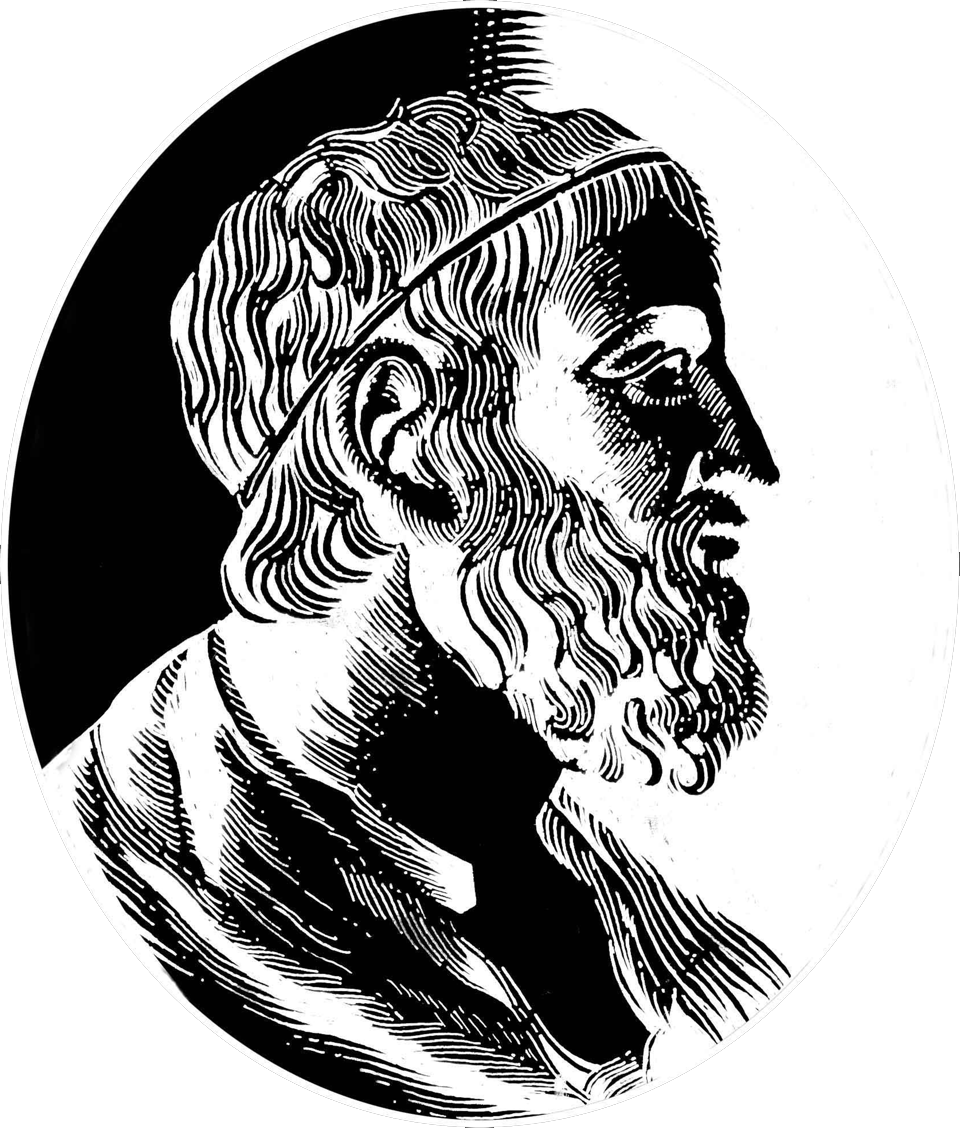
\includegraphics[height=2cm]{imelogo}\\[0.2cm] Department of Computer Science \\ University of São Paulo}

\begin{document}

\maketitle

%------------------------------------------------------------------------------
\begin{frame}{1990}
  \begin{figure}[ht]
    \centering
    
\includegraphics[width=0.5\textwidth, keepaspectratio=true]{images/1990.png}
  \end{figure}
\end{frame}

\begin{frame}{1990}
  \begin{columns}[T]
    \begin{column}{.5\textwidth}
      \begin{figure}[ht]
        \centering
        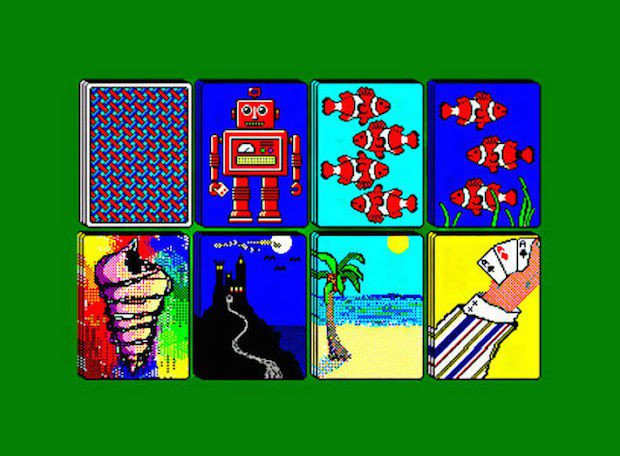
\includegraphics[width=0.6\textwidth, keepaspectratio=true]{images/1990_1.jpg}
      \end{figure}
      \begin{figure}[ht]
        \centering
        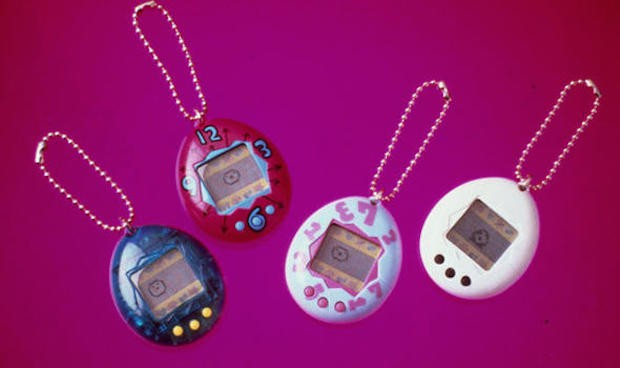
\includegraphics[width=0.5\textwidth, keepaspectratio=true]{images/1990_2.jpg}
      \end{figure}
    \end{column}

    \hfill
    \begin{column}{.5\textwidth}
      \begin{figure}[ht]
        \centering
        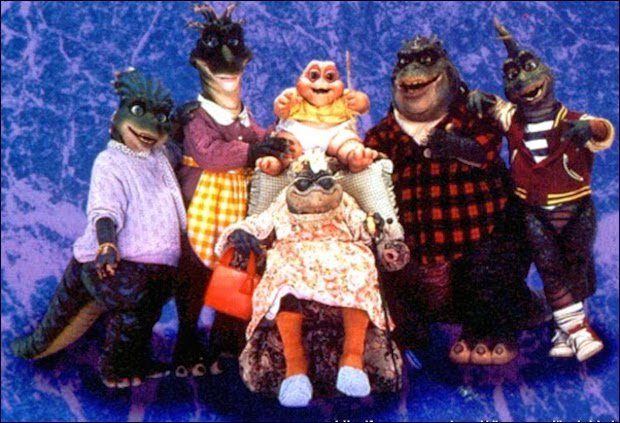
\includegraphics[width=0.5\textwidth, keepaspectratio=true]{images/1990_3.jpg}
      \end{figure}
      \begin{figure}[ht]
        \centering
        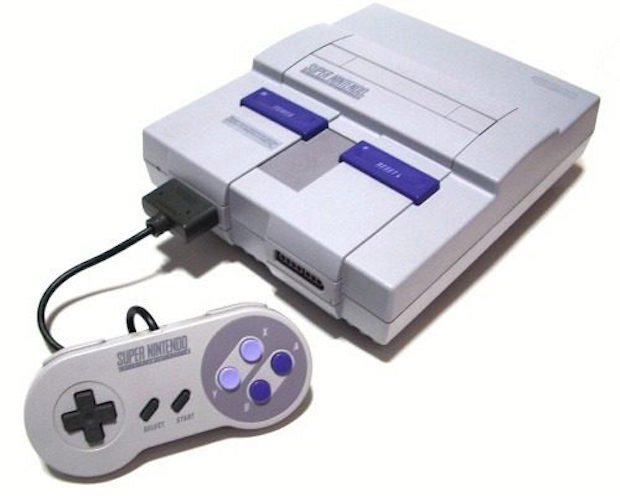
\includegraphics[width=0.5\textwidth, keepaspectratio=true]{images/1990_4.jpg}
      \end{figure}
    \end{column}
  \end{columns}
\end{frame}

\begin{frame}{1990}
  \begin{columns}[T]
    \begin{column}{.5\textwidth}
      \begin{figure}[ht]
        \centering
        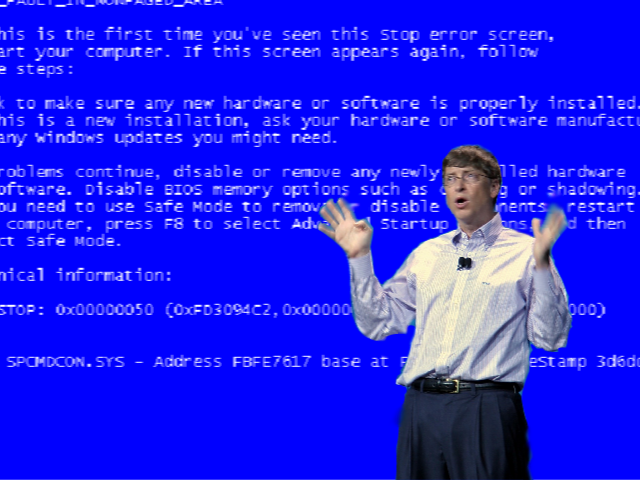
\includegraphics[width=0.8\textwidth, keepaspectratio=true]{images/1990_5.png}
      \end{figure}
    \end{column}

    \hfill

    \begin{column}{.5\textwidth}
      \begin{figure}[ht]
        \centering
        
\includegraphics[width=0.8\textwidth, keepaspectratio=true]{images/dial-up.jpg}
      \end{figure}
    \end{column}
  \end{columns}
\end{frame}

\begin{frame}{1990}
  \metroset{block=fill}
  \begin{alertblock}{Communication tools}
    \begin{itemize}
      \item Telnet
      \item RSH
      \item X
    \end{itemize}
  \end{alertblock}
\end{frame}

\begin{frame}{1990}
  \begin{figure}[ht]
    \centering
    
\includegraphics[width=0.6\textwidth, keepaspectratio=true]{images/wait.jpg}
  \end{figure}
\end{frame}

\begin{frame}{1990}
  \begin{figure}[ht]
    \centering
    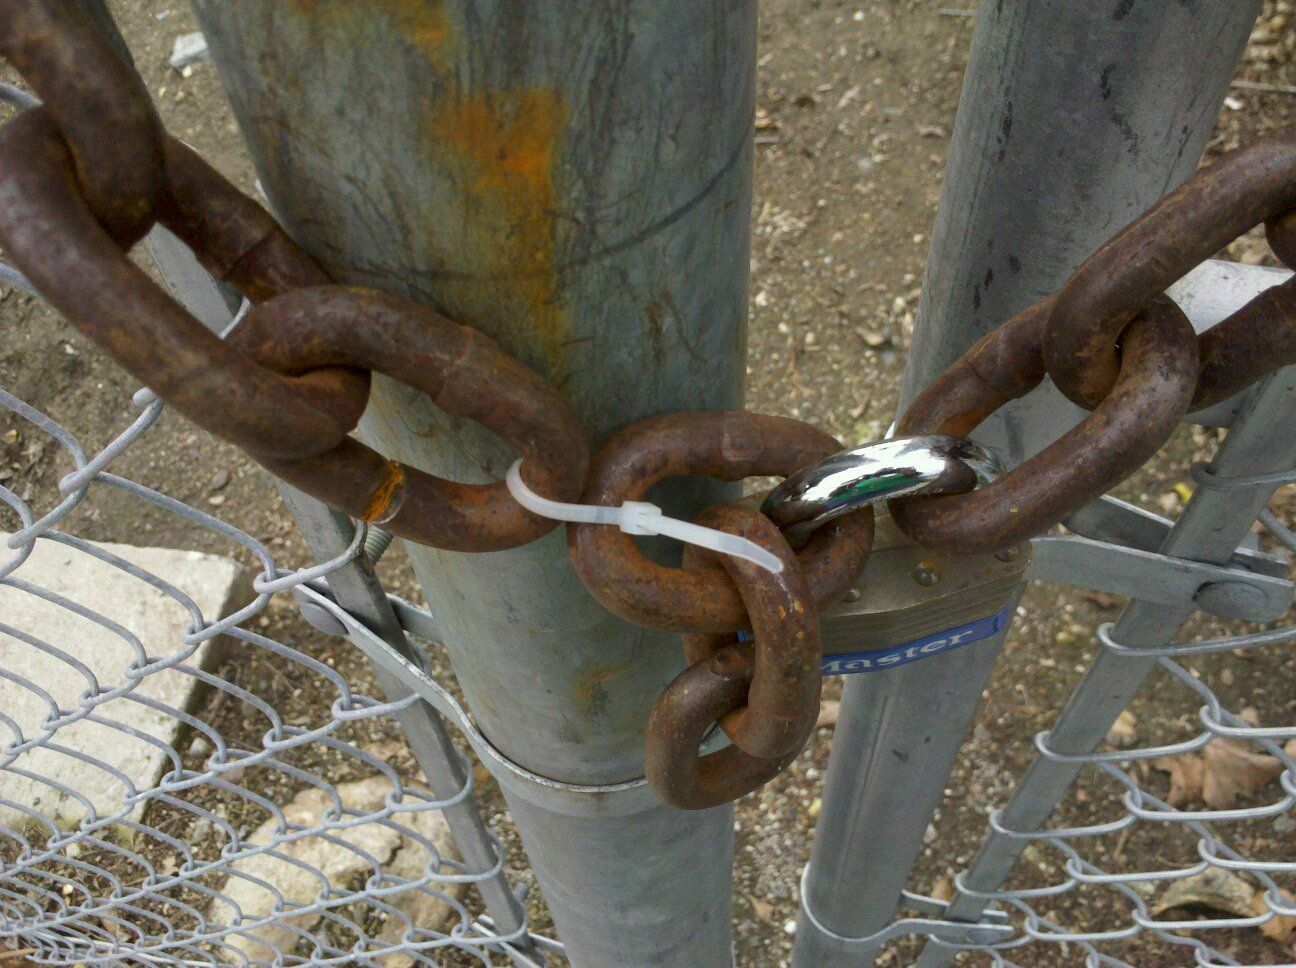
\includegraphics[width=0.7\textwidth, keepaspectratio=true]{images/secure_fail.jpg}
  \end{figure}
\end{frame}

\begin{frame}{Secure Shell}
  \begin{figure}[ht]
    \centering
    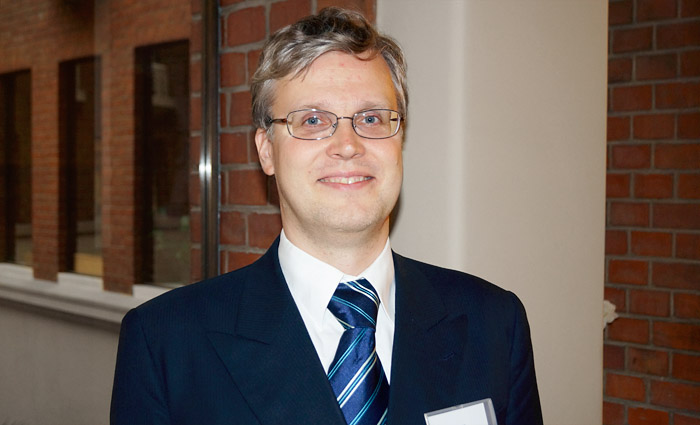
\includegraphics[width=0.6\textwidth, keepaspectratio=true]{images/TatuYlonen.jpg}
  \end{figure}
\end{frame}

\begin{frame}{Secure Shell - What is new?}
  \pause
  \begin{figure}[ht]
    \centering
    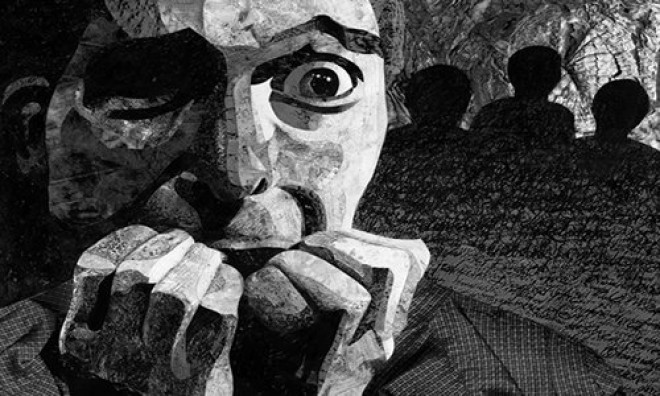
\includegraphics[width=0.8\textwidth, keepaspectratio=true]{images/paranoia.jpg}
  \end{figure}
\end{frame}

\begin{frame}{Heavily based on - RSA}
  \begin{figure}[ht]
    \centering
    
\includegraphics[width=0.8\textwidth, keepaspectratio=true]{images/rsa.png}
  \end{figure}
\end{frame}

\begin{frame}{RSA patents}
  \begin{figure}[ht]
    \centering
    
\includegraphics[width=0.6\textwidth, keepaspectratio=true]{images/wait.jpg}
  \end{figure}
\end{frame}

\begin{frame}{2000 - RSA patents expired}
  \begin{figure}[ht]
    \centering
    
\includegraphics[width=0.7\textwidth, keepaspectratio=true]{images/2000.png}
  \end{figure}
\end{frame}

\begin{frame}{Tatu's got to earn a living...}
  \pause
  \begin{figure}[ht]
    \centering
    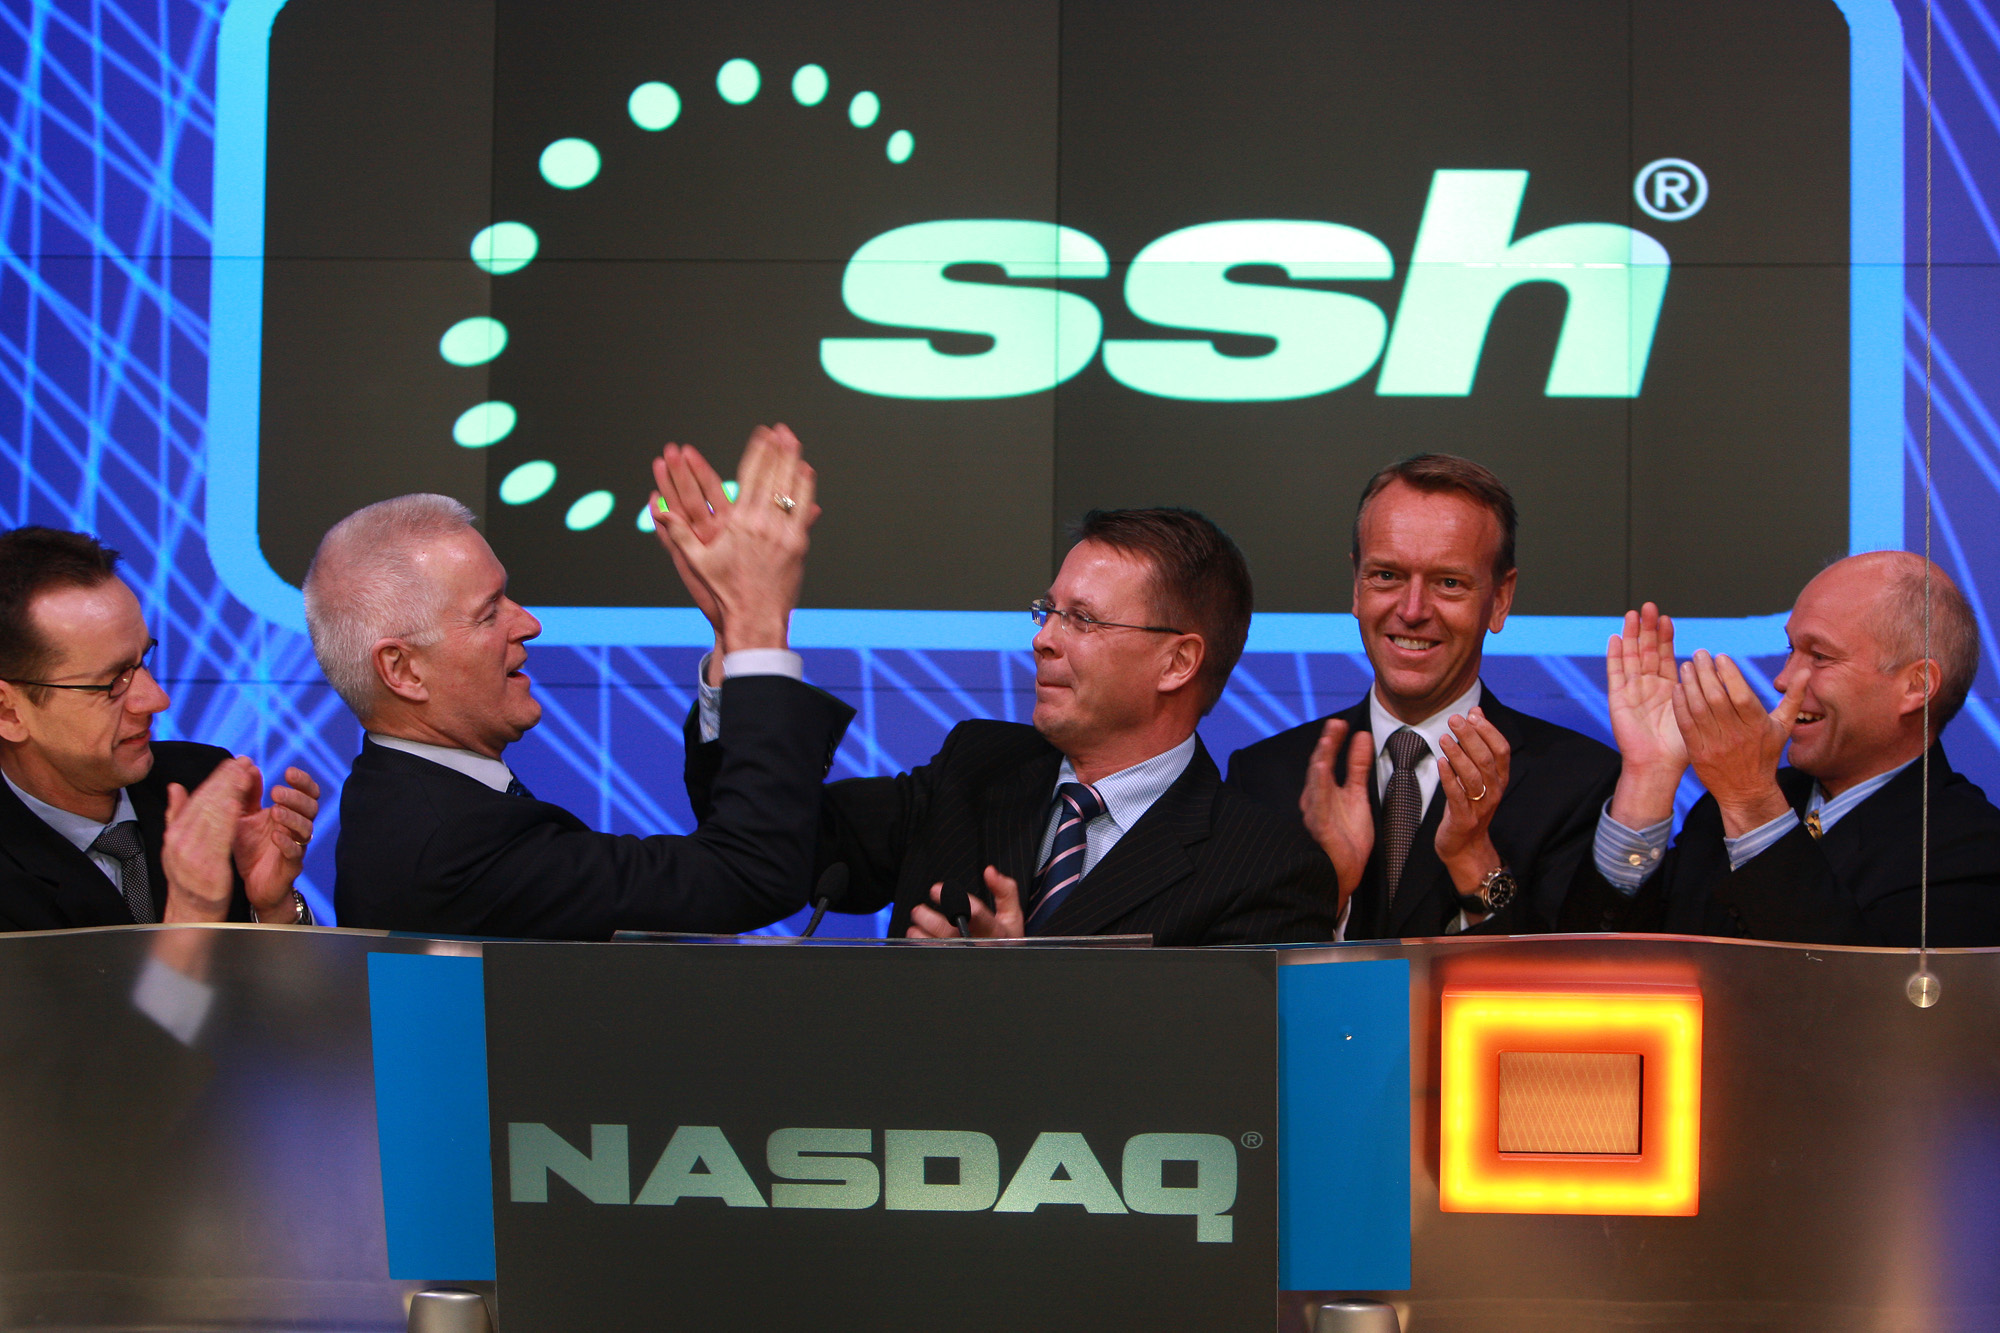
\includegraphics[width=0.7\textwidth, keepaspectratio=true]{images/ssh.jpg}
  \end{figure}
  \pause
  SSH VERSION 2.0 COMPLETELY CLOSED!
\end{frame}

\begin{frame}{New player: Theo De Raadt}
  \begin{figure}[ht]
    \centering
    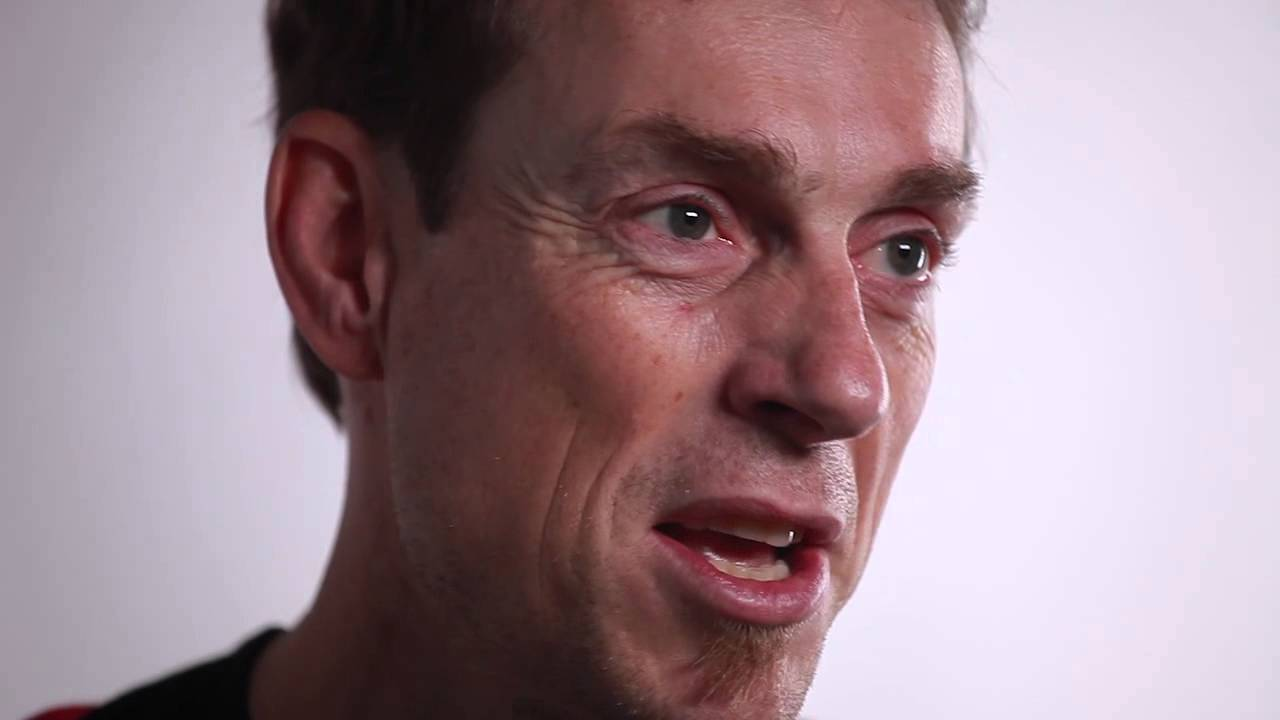
\includegraphics[width=0.7\textwidth, keepaspectratio=true]{images/theoDeRaadt.jpg}
  \end{figure}
\end{frame}

\begin{frame}{New player: Theo De Raadt and Björn Grönvall}
  \begin{figure}[ht]
    \centering
    
\includegraphics[width=0.7\textwidth, keepaspectratio=true]{images/openbsd.png}
  \end{figure}
\end{frame}

\begin{frame}{OpenSSH! It's alive!}
  \begin{figure}[ht]
    \centering
    
\includegraphics[width=0.5\textwidth, keepaspectratio=true]{images/openssh.jpg}
  \end{figure}
  \begin{itemize}
    \item Auditability
    \item Portability enhancements
  \end{itemize}
\end{frame}

\begin{frame}{Openssh Source}
  \metroset{block=fill}
  \begin{alertblock}{Project}
    \begin{itemize}
      \item git://anongit.mindrot.org/openssh.git (clone only)
      \item https://anongit.mindrot.org/openssh.git (web and clone)
    \end{itemize}
  \end{alertblock}
\end{frame}

%------------------------------------------------------------------------------
\section{That's it!}
\begin{frame}[standout]
   \begin{center}\ccbysa\end{center}
\end{frame}

\maketitle

\end{document}
